\section{Extreme Value Theory (EVT). }
\begin{frame}[plain]
        \vfill
      \centering
      \begin{beamercolorbox}[sep=8pt,center,shadow=true,rounded=true]{title}
        \usebeamerfont{title}\insertsectionhead\par%
        \color{oxfordblue}\noindent\rule{10cm}{1pt} \\
        \begin{itemize}
        \item Normal Choices are POT or Block Maxima, but these strategies require
              large amounts of data to converge~\cite{taleb2019much}.
        \item \texttt{skextreme}~\cite{skextremes} is an python package that implements these
              standard strategies.
        \item Taleb does present some solutions~\cite{taleb2019statistical}.
        \item As physical processes with understood causes, TCs
              and their storm surges are \textbf{grey not black
              swans}.\foonote{\url{http://news.mit.edu/2015/grey-swan-cyclones-storm-surge-0831}}
        \item Need to know bias between hourly to daily output.
        \end{itemize}
      \end{beamercolorbox}
      \vfills
\end{frame}


\begin{frame}{BM vs.\ POT Mathematics}
\begin{itemize}
  \item Both require domain of attraction condition~\cite{bucher2018horse}:

  \begin{enumerate}
    \item Either $\forall r \in \mathbb{N} \;\exists \;b_r \in \mathbb{R},\; \gamma\in \mathbb{R},\; a_r>0: $
      \begin{equation}
      \lim _{r \rightarrow \infty} F^{r}\left(a_{r} x+b_{r}\right)=\exp \left\{-(1+\gamma x)^{-1 / \gamma}\right\} \text { for all } 1+\gamma x>0
      \tag{BM}
      \end{equation}

    \item Or equivalently, there exists a positive function $\psi=\psi (t):$
      \begin{equation}
      \lim _{t \uparrow x^{*}} \frac{1-F(t+\psi(t) x)}{1-F(t)}=(1+\gamma x)^{-1 / \gamma} \text { for all } 1+\gamma x>0
      \tag{POT}
      \end{equation}
   \end{enumerate}

   \item BM leads to Generalised Extreme Value (GEV) distribution,
         whereas POT leads to Generalised Pareto Distribution (GPD).

\end{itemize}
\end{frame}

\begin{frame}{Initial Block Maxima EVT }
  \begin{itemize}
    \item The Block Maxima method with the ORCA12
    \texttt{control-1950} seemed easier to initially implement.
    \item Whether POT or BM converges faster depends
          on the underlying distribution~\cite{bucher2018horse}.
    \item The input is the 101 yearly maxima for each of the points along the coast,
         relative to the deviation from the long term mean.
    \item I initially used two different BM modules in \texttt{skextreme}, but present the
          results of the more flexible GEV implementation.
  \end{itemize}
\end{frame}



    \begin{frame}{GEV Equations }
    \begin{itemize}
\item
\(
\operatorname{GEV}(\mu, \sigma, \xi):
\)
\(
\text{ location, } \mu \in \mathbb{R}
\text{; scale, } \sigma>0
\text{; shape, } \xi \in \mathbb{R}.
\)
\begin{eqnarray}
\operatorname{GEV}(x; \mu, \sigma, \xi)=&
\frac{1}{\sigma} \chi(x)^{\xi+1} e^{-\chi(x)};\\
\chi(x)=&\left\{\begin{array}{ll}
\left(1+\xi\left(\frac{x-\mu}{\sigma}\right)\right)^{-1 / \xi} & \text { if } \xi \neq 0 \\
e^{-(x-\mu) / \sigma} & \text { if } \xi=0
\end{array}\right.
\end{eqnarray}
\item The Gumbel distribution is a special case ($\xi=0$)
\begin{equation}
\operatorname{GUM}(x ; \mu, \sigma)=e^{-\frac{x-\mu}{\sigma}-e^{-(x-\mu) / \sigma}}
\end{equation}
\end{itemize}
\end{frame}


\begin{frame}{GEV New Orleans}
\vspace{-20pt}
    %\centering
 \begin{minipage}{1.0\textwidth}
\begin{figure}[htb!]
    \centering
    \includegraphics[width=1\linewidth]{../surge/plots/GEV_modelNO.pdf}
    \vspace{-25pt}
   \caption{Interesting transition - does this represent hurricanes?}
    \label{fig:}
\end{figure}
\end{minipage}
\end{frame}


\begin{frame}{GEV Point Near New Orleans}
\vspace{-20pt}
    %\centering
 \begin{minipage}{1.0\textwidth}
\begin{figure}[htb!]
    \centering
    \includegraphics[width=1\linewidth]{../surge/plots/GEV_modelPNO.pdf}
    \vspace{-25pt}
   \caption{c.\ identical winds to NO, but v.\ different
     responsiveness. }
    %\label{fig:}
\end{figure}
\end{minipage}
\end{frame}

\begin{frame}{GEV Miami}
\vspace{-20pt}
    %\centering
 \begin{minipage}{1.0\textwidth}
\begin{figure}[htb!]
    \centering
    \includegraphics[width=1\linewidth]{../surge/plots/GEV_modelMM.pdf}
    \vspace{-25pt}
   \caption{Fits Line well.}
    %\label{fig:}
\end{figure}
\end{minipage}
\end{frame}

\begin{frame}{GEV Models Along Coast}
\vspace{-20pt}
    %\centering
 \begin{minipage}{1.0\textwidth}
\begin{figure}[htb!]
    \centering
    \includegraphics[width=1\linewidth]{../surge/plots/skextreme_second_tactic.pdf}
    \vspace{-15pt}
   \caption{Confidence intervals not defined near Miami and Eastport. }
    %\label{fig:}
\end{figure}
\end{minipage}
\end{frame}


\begin{frame}{There is a physical maximum, given the climatology.}

\vspace{-30pt}
\begin{figure}[htb!]
    \centering
    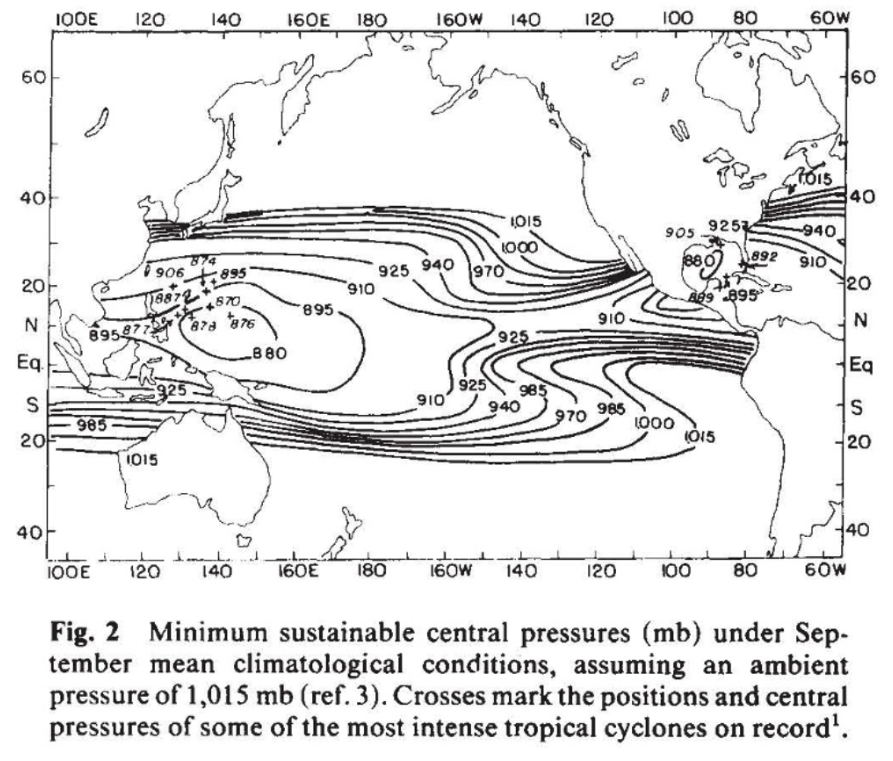
\includegraphics[width=0.8\linewidth]{images/hurricane-Emanuel-upper-bound.png}
    \vspace{-15pt}
   \caption{From Emanuel, Nature (1987)~\cite{emanuel1987dependence}~\footnote{Automatically Updated Version: \url{http://wxmaps.org/pix/hurpot}.} }
    \label{fig:}
\end{figure}
\end{frame}

\begin{frame}{So could we do something more intelligent?~\cite{taleb2019statistical}}
\vspace{-20pt}
    %\centering
 \begin{minipage}{1.0\textwidth}
\begin{figure}[htb!]
    \centering
    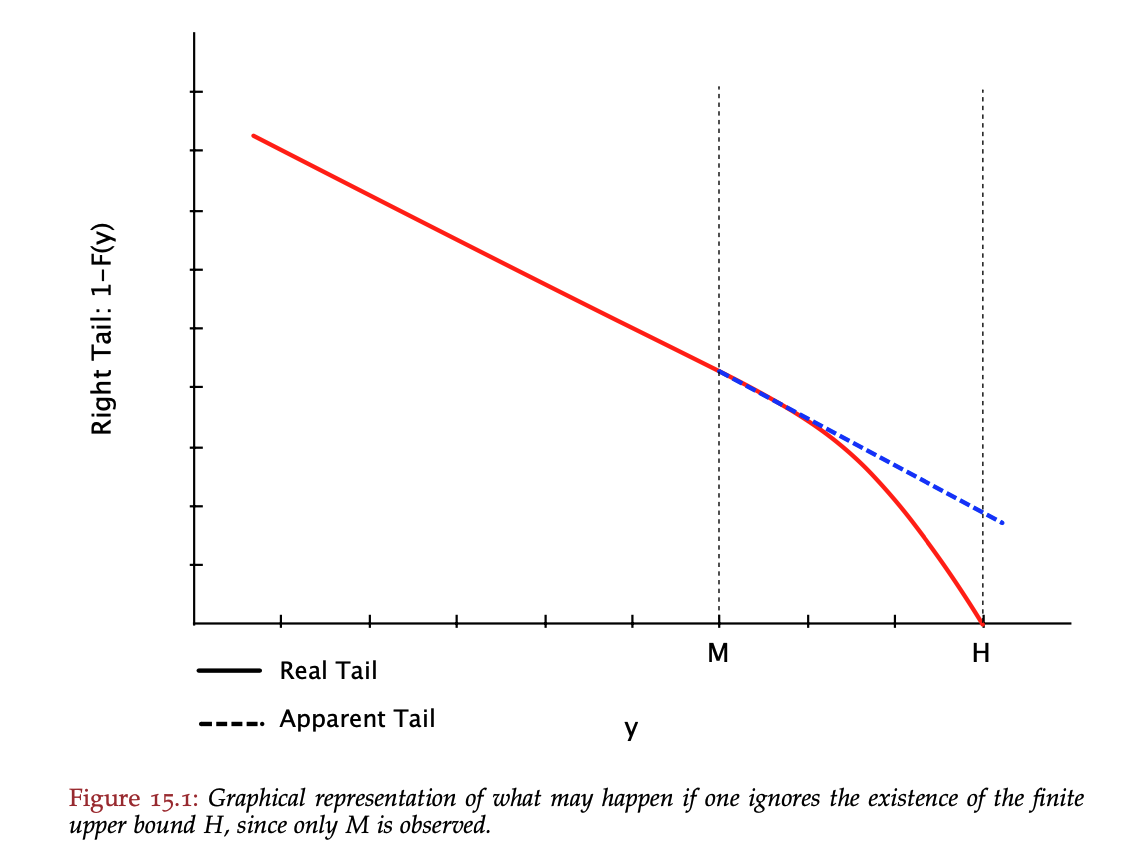
\includegraphics[width=1\linewidth]{images/nnt-upper-bound.png}
    \vspace{-15pt}

   %\caption{. }
    % \label{fig:}
\end{figure}
\end{minipage}
\end{frame}

\begin{frame}{Some Problems With Proposal}
\vspace{-15pt}
\begin{figure}
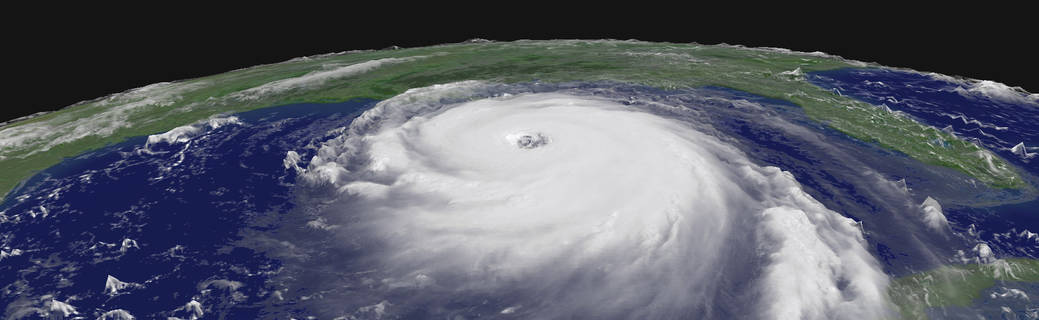
\includegraphics[width=\linewidth]{images/NASA-KATRINA-SIDEON.jpg}\\
Katrina just before landfall. \textit{Source: NASA}
\end{figure}
\vspace{-10pt}
\begin{itemize}
\item The minimum attainable TC central pressure varies between months and years.
\item The translation of this into the maximum winds requires some hurricane model
    (e.g. Holland~\cite{holland1980analytic, holland2010revised}).
\item
    The maximum velocity,
    \begin{equation}
    U_m = (\frac{B}{\rho e})^{0.5}(P_n-P_c)^{0.5}, \text{ is at }
    R_m = A^{1/B}.
    \end{equation}
\end{itemize}
\end{frame}


\begin{frame}{Some Problems With Proposal}
\vspace{-20pt}
\begin{figure}
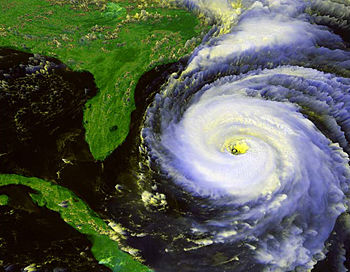
\includegraphics[width=0.4\linewidth]{images/hurricane_fran.jpg}\\
Fran before landfall. \textit{Source: NASA}
\end{figure}
\begin{itemize}
\item Once we know the maximum wind speed, we could combine it with the responsiveness,
     and some direction to see the theoretical maximum surge build up.
\item Both of these steps will make the theoretical maximum have a rather large
     (non-symmetric?) error envelope.

\end{itemize}
\end{frame}

\begin{frame}{Extratropical Cyclones (ECs) Limit Less Obvious}
\begin{figure}[htb!]
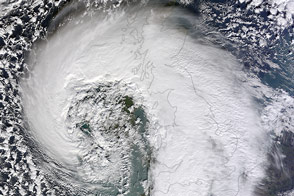
\includegraphics[width=0.4\linewidth]{images/ukstorm_tmo_2014043_tn.jpg}\\
EC over UK. \textit{Source: NASA}
\end{figure}
\begin{itemize}
\item Energy from the equator-pole temperature gradient
      drives heat engine~\cite{lorenz1960energy, holton2004introduction}.
\item In northern states  ECs pose a greater hazard, and are better sampled.
[But Hurricanes can still hit
 New England as in 1815 and 1938~\cite{emanuel2005divine}].
\item ECs may come on a continuous spectrum (with a limit?)
\end{itemize}
\end{frame}

\begin{frame}{Systematic Errors}
[(Effect on our estimate), source.]
\begin{enumerate}
\item ($-$) Coarsening of time to daily outputs.
\item ($-$) Lack of cyclogenesis  $\implies$ not enough TCs~\cite{tomassini2017interaction, williams2018met, FurtherInfo}.
\item ($\pm$) Parameterisation of heat transfer $\implies$ wrong strength?
\item ($\pm$) Parameterisation of wind stress $\implies$ wrong surge.
\item ($-$) SSH 4km out from the coast (centre of cell).
\item ($\pm$) No non-linear surge-tide interaction.
\item ($-$) No (or limited) wave buildup?
\item ($-$) Long TC return periods $> 100$~yrs (e.g. New England).
\end{enumerate}

\end{frame}
